%% bare_jrnl_compsoc.tex
%% V1.4a
%% 2014/09/17
%% by Michael Shell
%% See:
%% http://www.michaelshell.org/
%% for current contact information.
%%
%% This is a skeleton file demonstrating the use of IEEEtran.cls
%% (requires IEEEtran.cls version 1.8a or later) with an IEEE
%% Computer Society journal paper.
%%
%% Support sites:
%% http://www.michaelshell.org/tex/ieeetran/
%% http://www.ctan.org/tex-archive/macros/latex/contrib/IEEEtran/
%% and
%% http://www.ieee.org/

%%*************************************************************************
%% Legal Notice:
%% This code is offered as-is without any warranty either expressed or
%% implied; without even the implied warranty of MERCHANTABILITY or
%% FITNESS FOR A PARTICULAR PURPOSE! 
%% User assumes all risk.
%% In no event shall IEEE or any contributor to this code be liable for
%% any damages or losses, including, but not limited to, incidental,
%% consequential, or any other damages, resulting from the use or misuse
%% of any information contained here.
%%
%% All comments are the opinions of their respective authors and are not
%% necessarily endorsed by the IEEE.
%%
%% This work is distributed under the LaTeX Project Public License (LPPL)
%% ( http://www.latex-project.org/ ) version 1.3, and may be freely used,
%% distributed and modified. A copy of the LPPL, version 1.3, is included
%% in the base LaTeX documentation of all distributions of LaTeX released
%% 2003/12/01 or later.
%% Retain all contribution notices and credits.
%% ** Modified files should be clearly indicated as such, including  **
%% ** renaming them and changing author support contact information. **
%%
%% File list of work: IEEEtran.cls, IEEEtran_HOWTO.pdf, bare_adv.tex,
%%                    bare_conf.tex, bare_jrnl.tex, bare_conf_compsoc.tex,
%%                    bare_jrnl_compsoc.tex, bare_jrnl_transmag.tex
%%*************************************************************************


% *** Authors should verify (and, if needed, correct) their LaTeX system  ***
% *** with the testflow diagnostic prior to trusting their LaTeX platform ***
% *** with production work. IEEE's font choices and paper sizes can       ***
% *** trigger bugs that do not appear when using other class files.       ***                          ***
% The testflow support page is at:
% http://www.michaelshell.org/tex/testflow/


\documentclass[10pt,conference,onecolumn,compsoc]{IEEEtran}


\usepackage{hyperref}
\usepackage{enumitem}
\setlist[itemize]{leftmargin=3 cm}
\setlist[enumerate]{leftmargin=3cm}



% *** CITATION PACKAGES ***
%
\ifCLASSOPTIONcompsoc
  % IEEE Computer Society needs nocompress option
  % requires cite.sty v4.0 or later (November 2003)
  \usepackage[nocompress]{cite}
\else
  % normal IEEE
  \usepackage{cite}
\fi
% cite.sty was written by Donald Arseneau
% V1.6 and later of IEEEtran pre-defines the format of the cite.sty package
% \cite{} output to follow that of IEEE. Loading the cite package will
% result in citation numbers being automatically sorted and properly
% "compressed/ranged". e.g., [1], [9], [2], [7], [5], [6] without using
% cite.sty will become [1], [2], [5]--[7], [9] using cite.sty. cite.sty's
% \cite will automatically add leading space, if needed. Use cite.sty's
% noadjust option (cite.sty V3.8 and later) if you want to turn this off
% such as if a citation ever needs to be enclosed in parenthesis.
% cite.sty is already installed on most LaTeX systems. Be sure and use
% version 5.0 (2009-03-20) and later if using hyperref.sty.
% The latest version can be obtained at:
% http://www.ctan.org/tex-archive/macros/latex/contrib/cite/
% The documentation is contained in the cite.sty file itself.



% *** GRAPHICS RELATED PACKAGES ***
%
\ifCLASSINFOpdf
   \usepackage[pdftex]{graphicx}
    \graphicspath{ {images/} }
 
\else
 
\fi
% graphicx was written by David Carlisle and Sebastian Rahtz. It is
% required if you want graphics, photos, etc. graphicx.sty is already
% installed on most LaTeX systems. The latest version and documentation
% can be obtained at: 
% http://www.ctan.org/tex-archive/macros/latex/required/graphics/
% Another good source of documentation is "Using Imported Graphics in
% LaTeX2e" by Keith Reckdahl which can be found at:
% http://www.ctan.org/tex-archive/info/epslatex/
%
% latex, and pdflatex in dvi mode, support graphics in encapsulated
% postscript (.eps) format. pdflatex in pdf mode supports graphics
% in .pdf, .jpeg, .png and .mps (metapost) formats. Users should ensure
% that all non-photo figures use a vector format (.eps, .pdf, .mps) and
% not a bitmapped formats (.jpeg, .png). IEEE frowns on bitmapped formats
% which can result in "jaggedy"/blurry rendering of lines and letters as
% well as large increases in file sizes.
%
% You can find documentation about the pdfTeX application at:
% http://www.tug.org/applications/pdftex









% *** PDF, URL AND HYPERLINK PACKAGES ***
%
\usepackage{url}
% url.sty was written by Donald Arseneau. It provides better support for
% handling and breaking URLs. url.sty is already installed on most LaTeX
% systems. The latest version and documentation can be obtained at:
% http://www.ctan.org/tex-archive/macros/latex/contrib/url/
% Basically, \url{my_url_here}.




\begin{document}

\title{GambleMania}
%
%

% received ..."  text while in non-compsoc journals this is reversed. Sigh.

\author{Collin Winstead, Diego Arriaga% <-this % stops a space
}

\IEEEtitleabstractindextext{%
\begin{abstract}
GambleMania allows the user to play the popular casino game of blackjack against a computer-controlled dealer. Blackjack uses a custom design for the deck of cards the game uses. GambleMania does not require any real money to play; all money is virtual and has no real monetary value. Users will have their own accounts which will contain login information and the account's balance. This information will be managed with a database.
\end{abstract}

}


% make the title area
\maketitle



\IEEEdisplaynontitleabstractindextext

\IEEEpeerreviewmaketitle



\section{Introduction}


Our project is called GambleMania. It allows you to play the blackjack casino game. The player's balance will be saved in a database along with their login information. We decided to do this project because we thought it would be fun and require a good bit of research and work to finish. As for why we chose blackjack as the game to implement, it's because blackjack is a fairly simple game to learn and play.\\
\newline
As blackjack is fairly simple, it is easier to program than more complex games like poker. Our target audience is adults 18 years old and older because blackjack is a game that is typically played in casinos. We expect our audience to use our app simply for fun or to practice blackjack.\\



\subsection{Background}
Minimally, we expect the user to know how to play blackjack and be familiar with the terms used in blackjack. The goal of blackjack is to get the point value of your hand as close to 21 as possible without going over. The terms you should know are defined below.\\
\newline
\begin{itemize}
\item{Ante - the amount of money you bet before you play the game.}
\item{Blackjack - when your hand has a point value of 21.}
\item{Bust - when your hand has a point value greater than 21.}
\item{Push - when your hand and the dealer's hand have the same point value at the end of the dealer's turn.}
\item{Hit - deal another card to your hand.}
\item{Stand - end your turn.}
\item{Double down - double your ante bet and be dealt one, and only one, card to your hand.}
\item{Split - double your ante bet and split your hand into two hands. Both hands are dealt another card.}
\end{itemize}

\subsection{Impacts}
Although our project is very small and limited, if distributed the project could possibly have a cultural impact by getting more people into blackjack.

\subsection{Challenges}
Our biggest challenge was the logic behind blackjack. In blackjack, there are many conditions which you have to check for such as getting a blackjack or busting your hand. You have to check these conditions for both the user and the dealer, which further complicated the development of the game. This challenge was overcome by applying conditionals in places where they would only need to be checked once.\\
\newline
Before we began developing Gamblemania, we thought that programming the dealer's functions would be the most difficult challenge. However, this turned out to be almost trivial for blackjack because the dealer must play according to a strict guideline: hit until you get at least 17 or your hand is greater than the player's, then stand. This rule was handled by some simple conditionals and a loop.\\
\newline
Another challenge we faced was the ``split" functionality. Giving the user another hand doubles the amount of logic the program needs to run the game. By adding another hand, we now have to compare the user's hands seperately against the dealer's hand. This challenge has not been completely solved yet, as there are still some bugs with splitting. However, splitting works normally for the most part.

\section{Scope}
Firstly, the user should be able to navigate between pages by clicking a button on the page they are currently on. Users should be able to create accounts and log into them. The main menu should minimally allow the user to navigate between pages by clicking a button and return to desktop by clicking an exit button. The user must be able to play a game of blackjack with the rules of dealer stands on 17 and blackjack pays 3:2. Finally, all of the cards that you would use in blackjack must be designed.
\newline
Below is the future work we could do to expand GambleMania:\\

\begin{enumerate}
\item Add more games to the app.
\item Create a tutorial for each game for users who do not know how to play.
\item Make the main menu and game environments look better.
\item Networked gameplay
\end{enumerate}

\subsection{Requirements}
The basis of the base requirements stems from the rules of play for blackjack. There are also requirements that involve the UI design, some of which are simply required for a functional app and others are for a good-looking app. The non-functional requirements are based on how the user will interact with our app. These requirements are not necessarily required for the app to function, but are important for the users of our app.

\subsubsection{Functional}
\begin{itemize}
\item A button that exits the program in the main menu and in each of the games.
\item Buttons to navigate from the main menu to each of the games.
\item A back button in each game that navigates the user back to the main menu.
\item Game logic for each game.
\item A Microsoft Access database that stores user login information and user balances.
\end{itemize}

\subsubsection{Non-Functional}
\begin{itemize}
\item User login data is hashed.
\item The app should be responsive and perform well without any major dips in framerate.
\item When the user's balance is modified, it should be updated in the database as soon as possible.
\item The app should be flexible enough so that it is possible to scale it up in the future.
\end{itemize}

\subsection{Use Cases}
This section defines and ranks the use cases for our project. A table of use cases is shown in Table \ref{tab:useCaseIndex}.

\begin{table}
\centering
\begin{tabular}{|c|c|c|c|c|c|}
\hline
Use Case ID & Use Case Name & Primary Actor & Complexity & Priority \\
\hline \hline
1 & Log In & User & Easy & 1\\
\hline
2 & Sign Up & User & Med & 1\\
\hline
3 & Play Blackjack & User & Hard & 3\\
\hline
4 & Navigate the Main Menu & User & Easy & 2\\
\hline
5 & Exit the Program & User & Easy & 4\\
\hline
\end{tabular}
\caption{Use Cases}
\label{tab:useCaseIndex}
\end{table}

\subsubsection{Use Case 1: Log In}
See Figure \ref{fig:login}
\begin{enumerate}
\item User enters their username and password into the provided text fields.
\item User clicks submit.
\item If the username and password are found in the database, the user proceeds to the main menu. Otherwise, the user must keep entering the username and password until the username and password matches.
\end{enumerate}

\subsubsection{Use Case 2: Sign Up}
See Figure \ref{fig:login}
\begin{enumerate}
\item User enters the username and password for their new account.
\item User clicks submit.
\item Account is registered to the database and the user proceeds to the main menu with the new account. The new account will have a starting balance of \$1000.
\end{enumerate}

\subsubsection{Use Case 3: Play Blackjack}
See Figure \ref{fig:blackjack}
\begin{enumerate}
\item User places an ante bet.
\item User and dealer are dealt two randomly chosen cards. 
\item User is shown a maximum of four options: Hit, Stand, Double Down, and Split. Double Down is only shown on the first turn. Split is only shown on the first turn when the user has two cards of the same face.
\item If the user chooses the Hit option, the user will be dealt another card.
\item If the user chooses the Stand option, the dealer will begin their turn.
\item If the user chooses the Double Down option, the user will place a bet with the same value as the ante bet and be dealt another card. After this, the dealer's turn begins.
\item If the user chooses the Split option, the user's two cards will be split into separate hands. Each hand will be dealt another card, giving the user two hands with two cards each. The user can play each hand separately.
\item After the user's turn is over, the dealer's turn begins. The dealer uses the same options the user has.
\item After the dealer's turn is over the user's hand and the dealer's hand are compared. The hand with the closest point value to 21 is the winner.
\item After the game is over, the user may enter another bet or exit to the main menu.
\end{enumerate}


\subsubsection{Use Case 4: Navigate the Main Menu}
See Figure \ref{fig:main}
\begin{enumerate}
\item The user can click the ``Blackjack" button to go to the blackjack game screen.
\item The user can click the ``Log Out" button to log out of their account and go back to the log in/sign up screen.
\item The user can click the ``X" button at the top right corner of the screen to exit the program.
\end{enumerate}

\subsubsection{Use Case 5: Exit the Program}
See Figure \ref{fig:main}
\begin{enumerate}
\item The user can click the ``X" button at the top right corner of the main menu screen to exit the program.
\end{enumerate}

\newpage
\subsection{Interface Screenshots}

\begin{figure}[h]
\caption{Login/sign-up GUI}
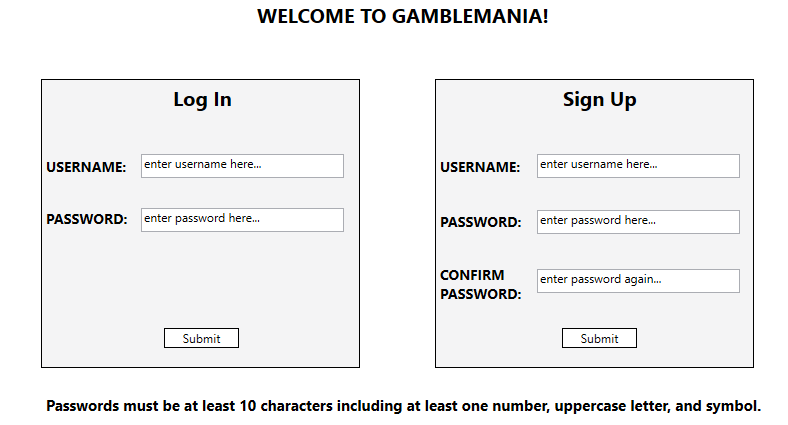
\includegraphics[scale=0.7]{Sign_Up}
\label{fig:login}
\centering
\newline The User will have the option to log in or Sign up, depending on whether or not they have an account.
\end{figure}

\begin{figure}[h]
\caption{Main menu GUI}
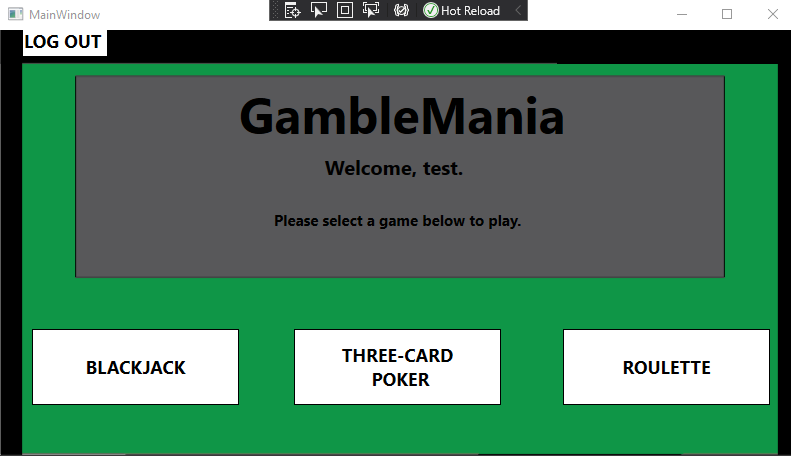
\includegraphics[scale=0.7]{Main_Menu}
\label{fig:main}
\centering
\newline The user will be logged in and will have the option to log out or play one of the three games displayed.
\end{figure}

\newpage

\begin{figure}[h]
\caption{Blackjack GUI}
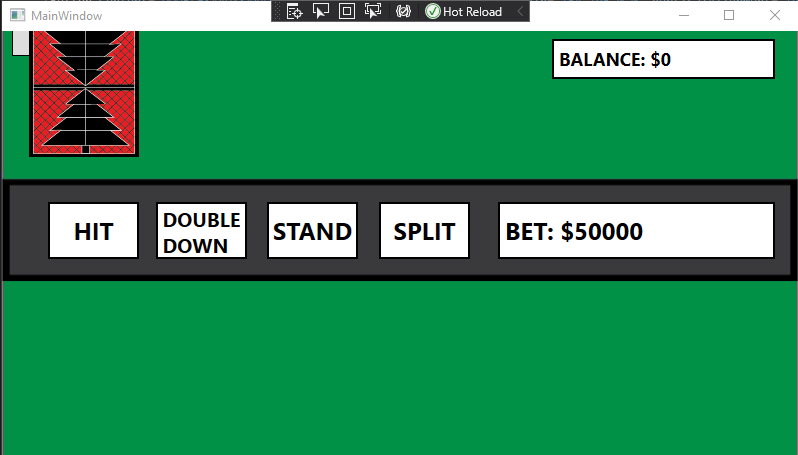
\includegraphics[scale=0.7]{Black_jack}
\label{fig:blackjack}
\centering
\newline The user will be handed two cards to gamble with and depending on the cards, the user will have the option to hit, double down, stand, or split, and have their points accumulated on the left and their balance on the top right with the current bet right under.
\end{figure}

\newpage

\section{Timeline}
\noindent
Below is the timeline of the project. This timeline is accurate up until 11/11. We were unfortunately delayed this week due to other events and could not work on the project. From then on, we were behind schedule and were not able to implement three-card poker and roulette as a result.\\
\newline
8/27 - Finding partners.\\
9/2 - Formed a team.\\
9/9 - Created a rough draft of the project proposal.\\
9/16 - Designed a plan of action for the project.\\
9/23 - Worked on the GUI mockups and the Requirements and Use Cases sections of the project proposal.\\
9/30 - Updated the GUI mockups.\\
10/7 - Researched potential design patterns for the project.\\
10/14 - Modified the Use Cases section of the project proposal.\\
10/21 - Midterms\\
10/28 - Added the Timeline and Project Structure \& UML Outline sections. Begin implementing the login/sign-up screen and database.\\
11/4 - Begin work on blackjack and three-card poker. Login/sign-up should be done by this point.\\
11/11 - We should be about halfway done with blackjack and three-card poker by this point.\\
11/18 - Begin work on roulette. Blackjack and three-card poker should be done by this point.\\
11/25 - Begin work on the presentation and work on stretch goals such as the tutorials.\\
12/2 - Demo the project. The project should be finished by this point.\\

\section{Project Structure}
\noindent
This section covers the general structure of our app. We designed our project's structure to be flexible and expandable. We made our project modular by using pages, which can be swapped in and out as needed. This means new pages can be added and removed very easily, and one page does not necessarily depend on another. Another way we made our project modular is that some of the classes we used in the Blackjack\_Page can be used in another card game. These classes are the CardFactory class, the card struct, and the CardType enum. All of these classes can be applied to a different card game.

\subsection{UML Outline}
\noindent
This section provides a UML outline of the project (see Figure \ref{fig:outline1} and Figure \ref{fig:outline2}). The outline was too big for one picture, so we had to separate it into two parts.\\
\newline
The project's structure hinges on a MainWindow object. The window has an object called a Frame that holds the page the user is currently on. At launch, the frame contains the log in/sign up page. To navigate between pages, we simply set the frame's content to a new instance of the page we want to navigate to. For each of the following pages, a reference to this frame is passed.\\
\newline
The log in/sign up page connects to the MS Access database through OleDb to log a user in or create an account for them. This page has two main methods: LoginSubmit\_Click and SignUpSubmit\_Click. As their names imply, these methods handle log ins and sign ups respectively.  LoginSubmit\_Click hashes whatever the user entered into the username and password fields on the page and compares them to every account in the database. If a match is found, then the user is logged in with that account. If not, the user is prompted to try again. SignUpSubmit\_Click
checks the validity of the username and password the user submitted and creates a new account in the database for the user if they are valid. ``Valid" in this case is when the password is at least 10 characters long and contains at least one uppercase letter, symbol, and number. The password must also match what the user entered in the ``Confirm password" text box. The username must not already be registered to another account.\\
\newline
The main menu page serves as a hub for navigation to other pages. Currently you can only navigate to the blackjack page and log out, but there is room for expansion when we get to that point. The two methods of this class, Black\_Jack\_Button\_Click and log\_out\_btn\_Click serve this purpose. They siimply navigate the user to the appropriate page.\\
\newline
The bet page does exactly what it implies: it allows the user to place a bet before they get into the game. Whenever the user enters a bet, the an event is raised that calls bet\_input\_TextChanged. This method validates the bet the user typed into the textbox. If the bet is valid, the user may click the submit button and navigate to their chosen game. The functionality for this is handled by submit\_btn\_Click.\\
\newline
The blackjack page is where the blackjack game is played. This class has several methods. There are four methods that represent actions the user can take in the game. These actions are hit, stand, double down, and split. There are four buttons that handle the logic behind these actions. Double down and split are only available on the player's first turn after they are dealt their starting hand. There are five methods in this class that deal with the functionality of the game. The first is checkHand, which checks the state of the given hand and returns that state as a string. So if the user has a blackjack, it will return ``blackjack." It will return the point value of the hand if the hand has no special state. A similar type of method is the insertCard method. This method simply adds a card to the given hand. The next method is Deal. This method initializes the game by dealing two random cards to the player and dealer. This method also handles blackjacks when needed. When the player clicks the stand button, dealerPlay is called. This method handles the logic behind the dealer's turn. This is made easy by the fact that the dealer must follow certain rules. The final functionality method is the play\_btn\_Click method. This method reveals the page content and calls Deal, which initializes the game. The last method in this class is the exit\_btn\_Click method, which simply closes the application.\\
\newline
Inside of the blackjack page class are three other classes: CardFactory, a card struct, and the CardType enum. The card struct defines what a card is. It contains three primitive values: ``value", ``suit", and ``face." ``value" is the amount of points a card is worth. ``suit" is the suit of the card (e.g. hearts). ``face" is what is displayed on the card (e.g. `K' for a King). CardType defines every card in a standard deck of cards (52 cards in total). CardFactory is an implementation of the Factory Method design pattern. Its role is to create a card object given a CardType.

\begin{figure}[h]
\caption{The Blackjack Page UML}
\centering
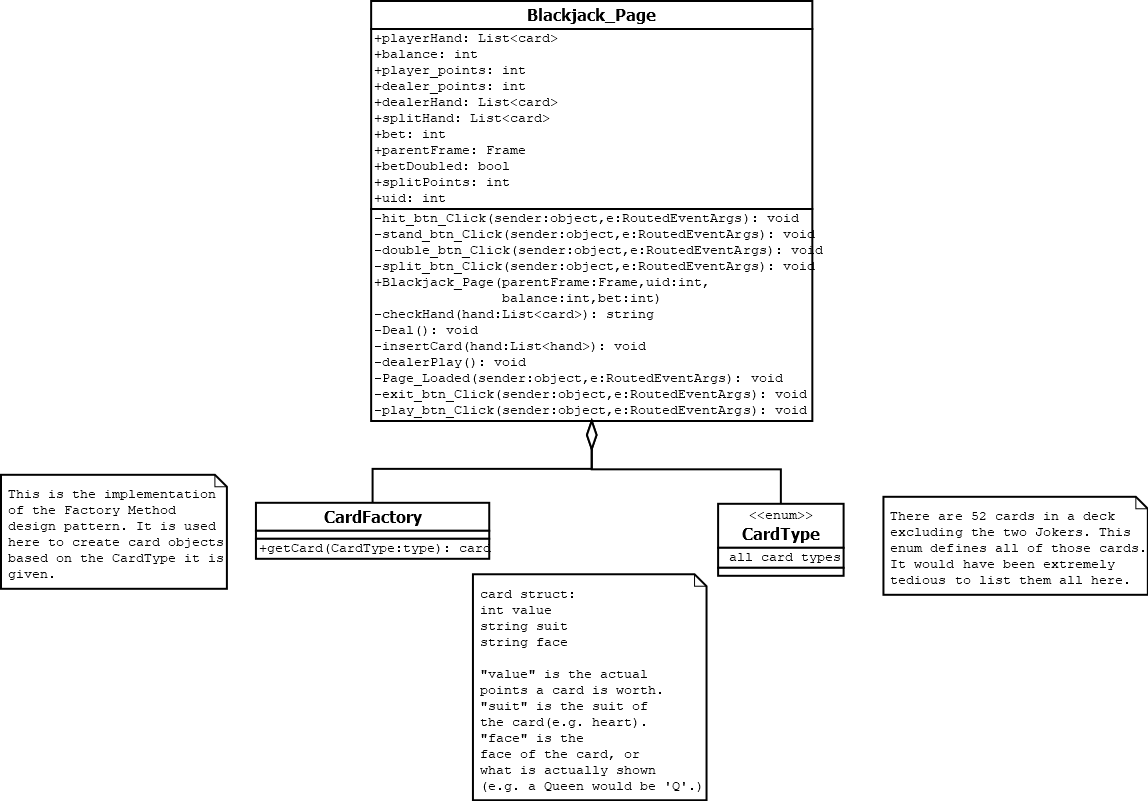
\includegraphics[scale=0.45]{Blackjack_UML}
\label{fig:outline1}
\centering
\end{figure}

\begin{figure}[h]
\caption{UML Outline}
\centering
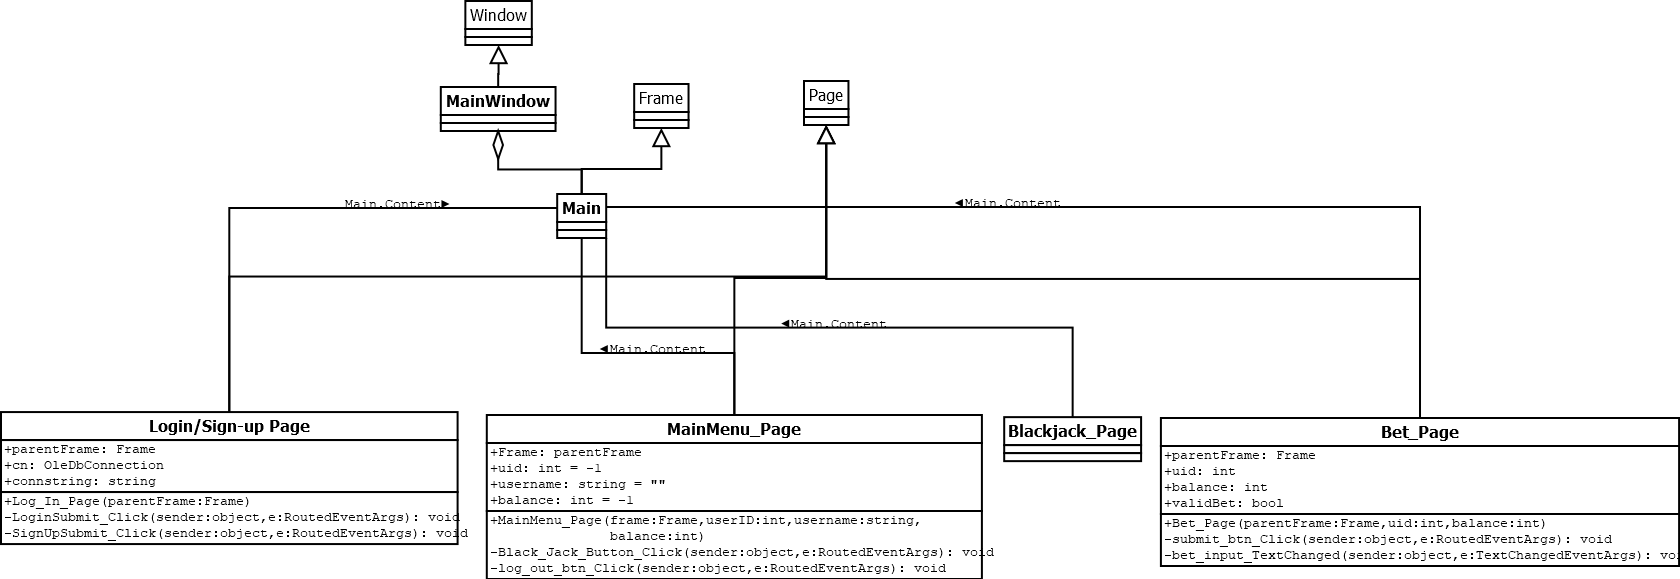
\includegraphics[scale=0.33]{whole}
\label{fig:outline1}
\centering
\end{figure}



\subsection{Design Patterns Used}
We used the Factory Method creational pattern and the Façade structural pattern for this project. We used the Factory Method to create objects that represent cards in our game. We chose to use this pattern because we needed a method of generating many different variations of the same object, and the Factory Method does that well. We used Façade to make playing the game much easier for the user. All the user needs to do  to control the game's subsystems is click some buttons.

\section{Results}
Looking back on the project, we managed to create a functional app with the limited time we had. As we developed the app, we discovered that our structure would definitely not work, so we had to quickly adapt to the changes in the structure. For example, we had planned to use a NavigationWindow as our method of navigation, but we discovered that it did not support the UI elements we needed to implement. Although there was probably a way around this, we found Pages to be easier to use. There is definitely room for improvement and expansion in the app, which is described in the Future Work section. As for our accomplishments, firstly we created a functional, albeit simple, user authentitication system using a Microsoft Access database. Second, we implemented user balances in the database. Finally, we created a functional blackjack game. Given more time, we could make many more accomplishments.


\section{Future Work}
In the future, we would like to expand the scope of our app to include the other games we originally planned to include: three-card poker and roulette. Another game we could potentially implement is  Texas Hold'em style poker game that can be played over the internet. Unfortunatley, due to time constraints we were only able to implement blackjack into the app. Finally, we would like to implement a tutorial page that contains tutorials for each game. 
% that's all folks
\end{document}
